%----------------------------------------
% Write your notes here
%----------------------------------------
\section{Part 1}
\subsection{Conduct 5\% margin of error}
\begin{documents}
\ITEM{\textbf{5\% margin}} margin of error means 5\% standard error or 5\% standard deviation in sampling distribution for the mean.
\\\\
\ITEM{\textbf{Given 5\%}} margin of error, 100 samples are needed. However,if the standard error is large such as 10\%, less samples will need. Following R codes has provided to demonstrate.\\\\
\ \# flip n times p=0.5
\\rbinom(n,1,p)\\
\#estimate p by measuring the fraction of heads \\
mean(rbinom(n,1,p)\\
\# repeat this 100,000 times\\
 p\_hat\<-\ replicate(1e5,mean(rbinom(n,1,p))\\
 \# look\enspace at\enspace a\enspace histogram\enspace of\enspace the\enspace estimates\\
 hist(p\_ hat)\\
 \# compute\enspace the\enspace standard\enspace deviation\enspace of\enspace the\enspace estimates\\
sd(p\_hat)\\


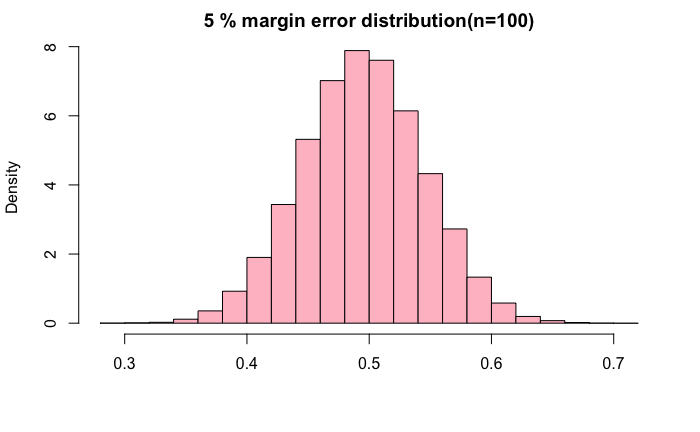
\includegraphics[width=12cm]{figures/ddg}

\end{documents}

\subsection{Apply Central Limit Theorem to Binomial Distribution}

\begin{documents}

\begin{equation} Var(\dfrac{1}{n} \sum_{i=0}^n X{i}) =\dfrac{1}{n^2}Var(\sum_{i=0}^n X{i}) = \dfrac{1}{n^2}(\sum_{i=0}^n Var (X{i}))=\dfrac{p(1-p)}{n}
\end{equation}
As a result, the number of sampling can be calculated by following way\\
\begin{equation}
S=SD(\dfrac{1}{n} \sum_{i=0}^n X{i})=\sqrt{\dfrac{p(1-p)}{n}}
\end{equation}

\begin{equation}
n=\dfrac{p(1-p)}{S^2}
\end{equation}
\end{documents}

\section{Part 2}
\subsection{Why Counting}

\begin{notes}
\ITEM{\textbf{Traditionally}} difficult to obtain reliable estimates due to small sample sizes or sparsity. \\\\
for example, (100age x 2sex x 5race x 3 party)=3,000 groups\\
As we know, 100 samples are needed to conduct 5\% margin error. For 3,000 groups, we need 100x3,000=300,000 samples. Apparently, it is almost impossible to conduct such experiment.  \\\\
\ITEM{\textbf{Potential solution}}\\
1.Combine large observations into fewer groups,which can cause of missing other important info. \\
2.Come up with more sophisticated methods generated by small samples.\\
3.\ITEM{\textbf{Obtain larger data samples }} by other ways and then count and divide to make estimates through its relative frequencies. \\\\
\ITEM{\textbf{Good and bad of large data }}\\\\
\ITEM{\textbf{Pros:}} move away from complicated and complex models generated by small samples to simpler models on large samples. \\
\ITEM{\textbf{Cons:}} Computationally challenging at large data.
\subsection{Learning to count}\\
\ITEM{\textbf{Claim:}} Solving the counting problem at scale enables you to investigate many interesting questions in the social sciences.\\\\ 
\ITEM{\textbf{R functions}}:\\
Split: Arrange observations into groups of interest.\\
Apply: Compute distributions and statistics within each group\\
Combine: Collect results across groups.\\\\
\ITEM{\textbf{Examples:}}



\usepackage{}
\usepackage{}

\begin{longtable}{}
\multirow{7}{*}{\begin{tabular}[c]{@{}c@{}}Group\\ a\\ b\\ a\\ c\\ c\\ b\end{tabular}} & \multirow{7}{*}{\begin{tabular}[c]{@{}c@{}}Value\\ 2\\ 3\\ 4\\ 10\\ 12\\ 9\end{tabular}} \\                                                &                                                   \\
                       &                                \\
\endfirsthead
\endhead
                           &                                                         \\
                                     &                                               \\
                                                &                                    \\
                                                       &                            
\end{longtable}
\\\\
\ITEM{\textbf{Several}} ways to approach the solution of finding the average per group. \\
1. First, find all a's and make a list of values such as (2+4)/2=3 for a's. Then, repeat for each group. With G*N steps and N space.\\
2.Run through observations and create list for each group.Then compute average each list. With N steps and N space\\
3.Create list for each group and keep running average instead of list.\\\\
\ITEM{\textbf{O(n*\ logn)}}: time for binary search and sorting algorithms.\\\\

\begingroup\centering \ITEM{\textbf{Movielens plots}}\\
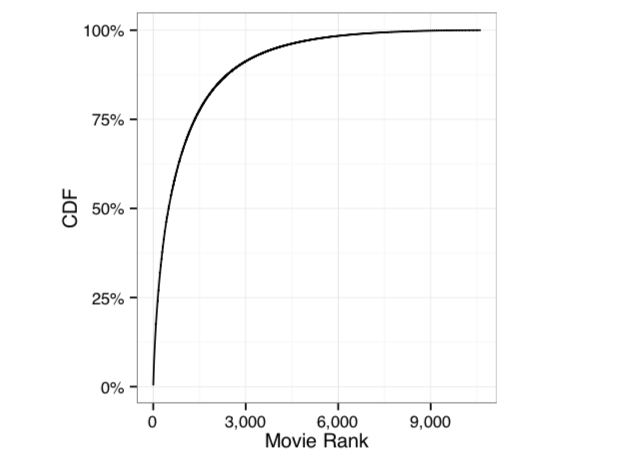
\includegraphics{figures/wee}\\

\endgroup According to the graph, majority rankings are from the most popular movies.\\

\begingroup\centering
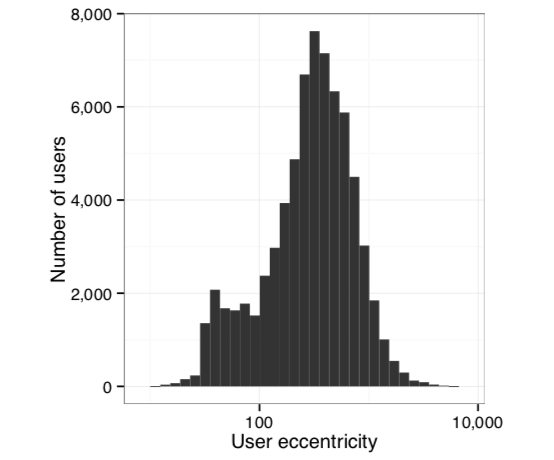
\includegraphics{figures/ddd}\\
\endgroup\\
Compute median movie rank as user eccentricity. However, when encountering a large data set, median is nearly impossible to find. \\\\
\ITEM{\textbf{Examples:}}\\\\
Ex1.\\
Take all your movies and look at popularity rank such as following\\
(3,7,100,120,9800)\\
The median rank as well as eccentricity is 100.\\\\
Ex2.\\
\begin{tabular}{cccc}
user & movie id & rating & ranking \\
1 & 37 & 1.5 & 8,000 \\
1 & 43 & 4.5 & 10 \\
1 & 2 & 3.0 & . \\
. & . & . & . \\
. & . & . & . \\
. & . & . & . \\
2 & 37 & . & 8,000
\end{tabular}
\end{notes}
\\
\section{Part 3}
\subsection{The group-by operation}
\ITEM{\textbf{Usually}} large data sets need large memory store. 
\begingroup\centering
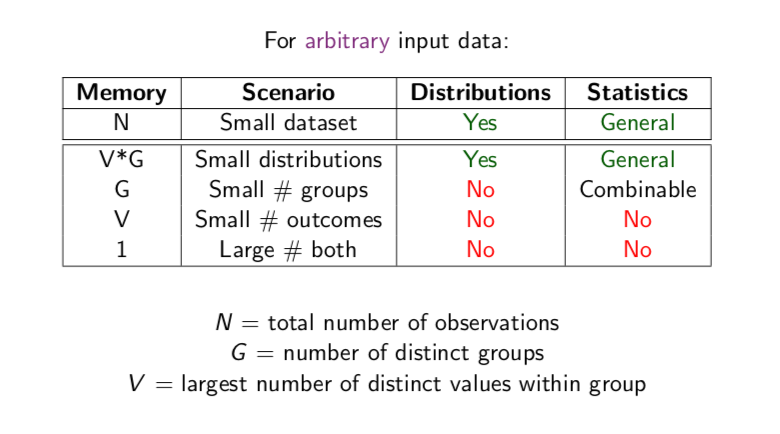
\includegraphics{figures/dda}\\
\endgroup\\
\noindent
\ITEM{\textbf{Combinable}}: means that all data is needed to compute median. \\
\ITEM{\textbf{Streaming}}: is required when full data-set exceeds available memory. It reads data one observation at a time, storing only needed state. It is also useful for computing a subset of within-group statistics with a limited memory footprint such as min, mean, variance but not median, requiring complete data set to compute.\\
\ITEM{\textbf{Median rating}} are used by both Netflix and YouTube.\\
\ITEM{\textbf{Mean rating}} is also utilized by YouTube, using streaming to compute combinable statistics. \\ 
\ITEM{\textbf{uniq-c}} in R: c(a,b,a,a,b,c) to c(a,b,a,b,c). Only delete next repeated occurrence. \\
\section{Part 4}
\subsection{Practice of Shell}
\ITEM{\textbf{Shell}} in Mac OS is called Terminal. \\
If you use Windows, you can try the built in bash/Ubuntu shell on Windows 10 or you can install it which includes bash and a terminal application by default. Linux also includes a working shell and terminal.\\
\ITEM{\textbf{Useful}} commands in terminal: curl -o [short name] [URL].
